% COMMANDS
\newcommand{\reporttitle}{Mandelbrot Set}
\newcommand{\ms}{\textit{Mandelbrot Set}}

\documentclass[english, 11pt]{tudscrartcl}
\iftutex
    \usepackage{fontspec}
\else
    \usepackage[T1]{fontenc}
\fi

% OPTIONS
\KOMAoptions{
    titlepage=true
}

\usepackage{babel}

% For math
\usepackage{amsfonts}
\usepackage{amsmath}
\usepackage{interval}
\newcommand{\floor}[1]{\left\lfloor #1 \right\rfloor}

% For tables
\usepackage{tabularx}
\usepackage{makecell}
\usepackage{multirow}
\usepackage{booktabs}

% For listings (code blocks)
\usepackage{listings}
\lstset
{ %Formatting for code in appendix
    basicstyle=\footnotesize\ttfamily,
    numbers=left,
    stepnumber=1,
    showstringspaces=false,
    tabsize=4,
    breaklines=true,
    breakatwhitespace=false,
}

% For references
\usepackage{nameref}
\usepackage{hyperref}

% For figures
\usepackage{graphicx}
\usepackage{rotating}
\usepackage{lscape}
\usepackage{calc}

% Spacings
\usepackage{enumitem}\setlist{noitemsep}
\newcommand{\setspacings}{
    \baselineskip=15pt
    \parskip=10pt
    \parindent=0pt
}

% TITLE
\faculty{Computer Science}
\institute{Institute of Systems Architecture}
\chair{Chair of Systems Engineering}
\date{\today}

\author{%
    Fritz Louis Wilke%
    \emailaddress*{E-Mail: fritz.wilke@tu-dresden.de}%
    \matriculationnumber{4536116}%
    \discipline{M. Sc. Computer Science}%
    \course{INF-MA-PR (graded)}%
}


\title{\reporttitle}
\subtitle{Lab: Concurrent and Distributed Systems}
\begin{document}

\setspacings
\maketitle

% The report content starts here
\clearpage
\setcounter{page}{1}

% INTRODUCTION
\section{Introduction}
\label{sec:introduction}

This report is part of the \textit{Concurrent and Distributed Systems Lab} which aims to test and improve practical knowledge about scalable, parallel programming.

\subsection{The Problem}
\label{ssec:problem}

The \ms{} is a set of complex numbers. It is mathematically defined by the recursive function $z_{n+1} = z_n^2 + c$ (1) with $z_0 = 0$ (2) for which $|z_n| < g$ holds. The threshold $g \in \mathbb{R}$ is a constant real number that is defined by $ g:= 2.0$ within this project. Complex numbers can be seen as a combination of two real numbers $r, i \in \mathbb{R}$ where $r$ represents the real part and $i$ the imaginary part. This representation simplifies the calculation of the \ms{} such that it only contains basic math.

The task is to write a program that creates an image of the \ms{} for a given amount of $rows$, $cols$ (resolution) and maximum amount of iterations $nn$. The iteration limit is needed or else the program would never terminate. To create an image of the \ms{} it must be mapped to a two dimensional plane. This is done by projecting each row of the image to the imaginary part and each column of the image to the real part of the $c$ from equation (1). This results in $p_{max} = rows*cols$ pixels and thus equations that need to be solved withing the range of the iterations limit.

\noindent In summary, the creation of the image contains the following steps:
\begin{enumerate}
    \item Select the next pixel $p < p_{max}$ to calculate. If there is no such p: \verb$terminate$
    \item Set complex number $z_0 := 0$
    \item Define $c$ depending on the $row$ and $column$ in which $p$ lays in
    \item Calculate equation (1) up to $z_{nn}$ (might be less if $\exists n: (n < nn) \land (|z_n| \ge 2.0)$)
    \item Set $p$ to \verb|'#'| if $|z_{nn}| < 2.0$ or to \verb|'.'| if not
\end{enumerate}


\subsection{Unoptimized Code Base}
\label{ssec:code-base}

An unoptimized version of the program was already implemented in \verb|C++|. This language was also used in the optimized program, but for evaluation purposes the program was also written in \verb|C| and \verb|C#|. The basic procedure of the unoptimized algorithm can be seen in Listing \ref{lst:pseudo-code-original}. It can be seen that this program is following the steps described in the \nameref{sec:introduction}. The unmodified code already contains one optimization in the while loop: The calculation may finish before reaching the iteration limit $nn$ if $|z_n| < 2.0$. This is due to the fact that once $z_n$ grows above the threshold $g := 2.0$ it will not shrink again. This saves a lot of calculations and therefore improves the overall performance of the program but it makes it especially hard to split up the work between multiple threads.

\begin{lstlisting}[caption={Pseudo Code of the unoptimized Algorithm}, label={lst:pseudo-code-original}, captionpos=b, frame=tb, float]
input: uint rows, uint cols, uint nn
output: char[]
begin
    let img = char[rows][cols]
    
    for r in 0..rows:
        for c in 0..cols:
            let z = complex(0, 0)
            let n = 0
            
            while |z| < 2.0 and n < nn:
                z = z*z + complex( c*2 / cols - 1.5, r*2 / rows - 1.0 )
                n = n + 1
            
            img[r][c] = (n == nn) ? '#' : '.'
    
    for r in 0..rows:
        for c in 0..cols: print( img[r][c] )
        print( '\n' )
end
\end{lstlisting}

The result is stored in an array of arrays of chars. To calculate it, the algorithm iterates over all rows and columns. The $z_n$ is then computed up to a maximum of $nn$ iterations. Depending on the amount of iterations needed, the pixel \verb|img[r][c]| is set. Finally, each character is printed to the standard output. The in Listing \ref{lst:pseudo-code-original} implemented algorithm has the complexity $\mathcal{O}(r*c*nn+r*(c+1))$ where $r$, $c$ and $nn$ are the given parameters for $rows$, $columns$ and \textit{iteration limit} respectively. The first part of the sum is derived from the actual calculation, the second from the printing of the result.


\section{Optimization Strategies}
\label{sec:strategies}

To improve the scalability of the shown algorithm, several strategies have been developed and tested. The hard part of developing scalable software (w.r.t. the amount of CPU cores) is to distribute the given workload equally between the CPU cores while still having a correct result in the end. The two most successful strategies are presented in the following sections.

\subsection{Strategy I: Shared Variable}
\label{ssec:strategy-i}

This strategy is very simple and easy to implement as it only needs one shared variable $p_{next}$ between the \textit{worker threads}, that holds the next pixel to work on. To prevent \textit{race conditions}, a \textit{mutex} is used for mutual exclusion when accessing the variable. Once a \textit{worker thread} needs more work, it locks the mutex, stores the content of $p_{next}$ in a thread local variable and increases $p_{next}$ by one. After that, the mutex is unlocked again to make $p_{next}$ available for other threads again.

This strategy provides dynamic work load distribution between the \textit{worker threads} while offering \textit{fairness} and prevent \textit{starving}. It fits the problem of this lab because the workload of the calculation of the \ms{} cannot be split up in a trivial way. This is due to the fact that the iterations needed to calculate each pixel may vary between $1$ and $nn$.

\noindent The strategy should be scalable and improve the performance for several reasons:
\begin{itemize}
    \item Several threads can do the work in parallel that was done by only 1 thread before
    \item Synchronization is only done once every pixel, for only a single, short access of the shared variable
    \item The time span in which the mutex is locked is a lot smaller than the time spent calculating
    \item Workload is dynamically distributed, thus every thread should have the same amount of work no matter how many pixels they work with
\end{itemize}


\subsection{Strategy II: I/O Queues}
\label{ssec:strategy-ii}

\begin{figure}[b]
   \centering
   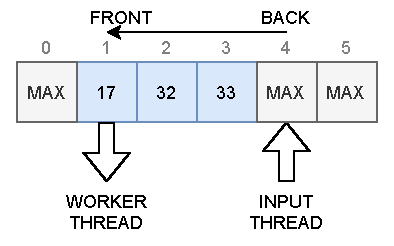
\includegraphics[width=0.45\textwidth]{mandelbrot/assets/input-queue.pdf}
   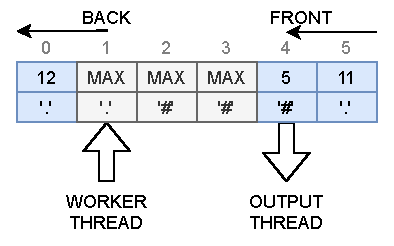
\includegraphics[width=0.45\textwidth]{mandelbrot/assets/output-queue.pdf}
 \caption{Example of an Input-Queue (left) and Output-Queue (right)}
 \label{fig:queues}
\end{figure}

This strategy is substantially different to the first one. The work is not pulled by the worker threads themselves but pushed to them through queues, making this solution more complex. The idea is to have again one \textit{worker thread} for each CPU and additionally two \textit{I/O threads} that distribute and collect the work and results respectively.

There is some overhead because of the I/O threads, which should decrease in relation to the amount of CPUs used. The performance reduction by the I/O threads is especially high when using one CPU because of the increased workload and cache usage of this single CPU. For each \textit{worker thread}, the \textbf{input thread} has an \textbf{input queue} and the \textbf{output thread} an \textbf{output queue}. If, for example, a worker provides a calculated pixel result in its output queue, only this cache line containing output results of this specific worker is invalidated. The only other thread that accesses this line is the output worker while the cache of the other workers stays valid since they do not know the queues of other \textit{workers}. The same applies for the input distribution. A graphical example of \textit{input-} and \textit{output queues} is shown in Figure \ref{fig:queues}. Note that these examples already contain some implementation specific details.

The input worker will iterate over all input queues of the worker threads, trying to fill them up, while the output worker keeps emptying the output queues. Having separate I/O queues for each thread involves one major advantage: no locking, no mutexes and no semaphores needed. This is possible because the queues are \textbf{unidirectional} and due to the \textbf{1:1 relation} between the I/O threads and the queues' worker thread. An input queue is always filled by the one input thread and emptied by a single worker thread, the output thread gets filled by a single worker and emptied by the output thread.

This strategy is scalable for the same reasons as \hyperref[ssec:strategy-i]{Strategy I}, but it has some additional advantages. The most important one is that this strategy does not need simultaneous access of many threads on the same shared variable. This can be a real problem when heaving a lot of threads.

\section{Implementation}
\label{sec:implementation}

This section presents the most important implementation details of the optimized program. At first, general improvements on the code are elaborated, which also affect the single thread performance. The latter subsection focuses on the improvements that have been made specifically for multithreading.

\subsection{General Improvements}
\label{ssec:general-improvements}

The improvement with the biggest effect is the simplification of the calculations. The while loop (line 11 in \hyperref[lst:pseudo-code-original]{Listing 1}) of the \ms{} calculation is the part of the program where the most computation time is spent. Optimizing this loop will have the biggest effect on the overall performance of the program.

The following improvements have been made on the code for the \ms{} calculation:
\begin{itemize}
    \item Substituting the addition of the freshly created complex number by a precalculated, per-pixel constant $c$
    \item Work directly on floats instead of using the class \verb|std::complex<float>|
    \item Optimizing the comparison $|z_n| < 2.0$ by squaring. The resulting comparison is $Re(z_n)^2 + Im(z_n)^2 < 4.0$
    \item Storing the already squared real and imaginary part of the above term and reusing them for calculating $z_n^2$ in the step
\end{itemize}

Further, smaller optimizations are:
\begin{itemize}
    \item Using one block of memory/one array instead of an array of arrays to store the resulting image in. This might improve cache access due to locality
    \item Using \verb$scanf()$, \verb$printf()$, \verb$fwrite()$ and \verb$fputc()$ instead of the \verb$std::cin$ and \verb$std::cout$ streams
    \item Using structs instead of any variables for the calculations and I/O management. The structs are aligned to start in a new cache line (at 64byte) and are padded to prevent any other threads to invalidate it
\end{itemize}


\subsection{Parallel Implementation}
\label{ssec:parallel_implementation}

\hyperref[ssec:strategy-ii]{Strategy II} was implemented as it is the more promising strategy. As already mentioned, C++ is used, together with the low level thread library \verb$pthread$. The basic workflow is like this:

\begin{enumerate}
    \item Read parameters from \verb$stdin$
    \item Create one \verb$img = new char[rows*cols]$ that will contain the result. Pixels are accessed via \verb$img[row*cols + col]$
    \item Create the \textit{input worker} thread that already starts to fill up the \textit{input queues} of the \textit{worker threads}
    \item Create as many \textit{worker threads} as the summed up \textit{thread concurrency} of all CPUs. This is given by the \verb$MAX_CPUS$ environment variable
    \item Create the \textit{output worker} that collects the results of each \textit{worker thread} from their \textit{output queues}
    \item Wait for the \textit{input worker} thread to finish and join it. Then join the \textit{output worker} thread
    \item Signal the \textit{worker threads} that there is no further input coming by setting the global \verb$bool done=true$
    \item Join all \textit{worker threads}
    \item Print the result
\end{enumerate}

On each thread creation, the parameters are given as a pointer to a struct. The structs are aligned to start with the beginning of a cache line (64 byte) and the important parts of them are padded such that they also fill up the full cache line. This should prevent unnecessary cache invalidation thus reducing cache misses. In fact, cache misses are pretty low for this implementation. A miss rate of 0.01\% has been measured on a 6 core (12 thread) computer with 19.50 MiByte cache, which makes it a bit more than half of the cache size of the evaluation system. But it is expected to have more cache misses with an increasing number of CPUs, since the \textit{I/O worker} threads have more caches to invalidate.

To provide maximum efficiency, the \textit{input-} and \textit{output queues} have been implemented as raw arrays of a fixed size, to match exactly one cache line. The \textit{input queues} consist of 16 \verb$uint32_t$ values which are initialized with \verb$UINT32_MAX$. They get filled up with pixel numbers which the corresponding \textit{worker thread} has to calculate. If the pixel number at the front of the queue is \verb$UINT32_MAX$, it means that the queue is empty and the \textit{worker thread} has to wait for more input. Once the value is not \verb$UINT32_MAX$ anymore, the \textit{worker thread} reads the pixel number, stores it in a thread local variable and changes the queue value to \verb$UINT32_MAX$ again. The pointer to the front of the queue has to be increased by one after this, to point to the next queue element. After that, the \textit{input worker} may store new pixel numbers in it again. Note that the \textit{worker thread} always works at the beginning of the queue, while the \textit{input worker} fills the queue up from the end, to provide a real \textit{FIFO} behaviour.

The \textit{output} queues are implemented in a similar way, but consist of 8 \verb$<uint32_t, char>$ pairs that represent one pixel value for a specific pixel number. To show that a field of the queue is empty, the pixel number is again set to \verb$UINT32_MAX$. A \textit{worker thread} fills up its \textit{output queue} from the back until it is full, the \textit{output worker} thread keeps emptying from the beginning. An example of the \textit{queues} can be seen in Figure \ref{fig:queues}. Note that they are shown with a length of 6 instead of the 16 and 8, which are the lengths used in the implementation.

Each beginning and end of a queue is stored in a thread local variable since the queue is only \textbf{written} by a single thread and \textbf{read} by another single thread. Thus it does not need any synchronization for them. Note that there still is implicit synchronization when reading or writing a queue depending on the pixel number that is stored at that queue position.

An identical implementation is done in C\# as well. The implementation only differs in one important aspect: on linux, it is not possible to bind a thread to a specific CPU (CPU affinity) using \textit{.Net}. We chose C\# to see how an interpreter copes with the given task.


\section{Evaluation}
\label{sec:evaluation}

\begin{table}[bt]
    \centering
    \begin{tabularx}{\textwidth}{clrrrrcX}
        \toprule
        
        &
        &
        &
        &
        \multicolumn{2}{c}{\thead{\textbf{Speedup@56}}} &
        &
        \\
        
        \cmidrule{5-6}
        
        \thead{\textbf{Lang.}} &
        \multicolumn{2}{c}{\thead{\textbf{Measurement}}} &
        \thead{\textbf{Time@56}\\\textbf{{[ms]}}} &
        \thead{\textbf{abs}} &
        \thead{\textbf{rel}} &
        \thead{\textbf{Git Hash}} &
        \thead{\textbf{Evaluation Log}} \\
        
        \midrule
        
        \multirow{3}{*}[-0.5em]{C++} &
        0: &
        Unmodified &
        207050 &
        1x &
        1x &
        \href{https://se-gitlab.inf.tu-dresden.de/FLWilke/cds-s-2021/-/blob/c4e204b77e805787b6aaa5fb318883e5395b5320/tasks/mopp-2017-t3-mandelbrot-set/mandelbrot_original.cpp}{\texttt{c4e204b7}} &
        \href{https://cds-lab.pages.se-gitlab.inf.tu-dresden.de/cds-s-2021/cds-website/logs/c75cb293de1ed36a6bb94494fd0b3b8f3b23c2290f5a165617ce8b8dc5681fe8/2021-04-30T20:17:30+02:00.html}{30.04.2021 20:17:30} \\
        
        \cmidrule{2-8}
        
        &
        1: &
        I/O Threads &
        2182 &
        86x &
        83x &
        \href{https://se-gitlab.inf.tu-dresden.de/FLWilke/cds-s-2021/-/blob/e0e78a6fff88e4338b6a0ca939ba820f52ae7f37/tasks/mopp-2017-t3-mandelbrot-set/mandelbrot.cpp}{\texttt{e0e78a6f}} &
        \href{https://cds-lab.pages.se-gitlab.inf.tu-dresden.de/cds-s-2021/cds-website/logs/c75cb293de1ed36a6bb94494fd0b3b8f3b23c2290f5a165617ce8b8dc5681fe8/2021-04-28T20:17:08+02:00.html}{28.04.2021 20:17:08} \\
        
        \cmidrule{2-8}
        
        &
        2: &
        + Simplified &
        \textbf{263} &
        \textbf{716x} &
        73x &
        \href{https://se-gitlab.inf.tu-dresden.de/FLWilke/cds-s-2021/-/blob/43c3df53ecea64e10961dca8c41823ed766cba4c/tasks/mopp-2017-t3-mandelbrot-set/mandelbrot.cpp}{\texttt{43c3df53}} &
        \href{https://cds-lab.pages.se-gitlab.inf.tu-dresden.de/cds-s-2021/cds-website/logs/c75cb293de1ed36a6bb94494fd0b3b8f3b23c2290f5a165617ce8b8dc5681fe8/2021-05-09T16:17:19+02:00.html}{09.05.2021 16:17:19} \\
        
        \midrule
        
        \multirow{2}{*}[-1em]{C\#} &
        0: &
        Unoptimized &
        63332 &
        1x &
        1x &
        \href{https://se-gitlab.inf.tu-dresden.de/FLWilke/cds-s-2021/-/blob/2fc35a6adcf1e26c341b9d8979d035154efd6b5f/tasks/mopp-2017-t3-mandelbrot-set-c\%23-unoptimized/Program.cs}{\texttt{2fc35a6a}} &
        \href{https://cds-lab.pages.se-gitlab.inf.tu-dresden.de/cds-s-2021/cds-website/logs/c75cb293de1ed36a6bb94494fd0b3b8f3b23c2290f5a165617ce8b8dc5681fe8/2021-05-12T00:16:54+02:00.html}{12.05.2021 00:16:54} \\
        
        \cmidrule{2-8}
        
        &
        2: &
        \makecell{I/O Threads \\+ Simplified} &
        452 &
        146x &
        \textbf{1798x} &
        \href{https://se-gitlab.inf.tu-dresden.de/FLWilke/cds-s-2021/-/blob/3ab6c9f1111b224f0546b0ccb107a86ab7786720/tasks/mopp-2017-t3-mandelbrot-set-c\%23/Program.cs}{\texttt{3ab6c9f1}} &
        \href{https://cds-lab.pages.se-gitlab.inf.tu-dresden.de/cds-s-2021/cds-website/logs/c75cb293de1ed36a6bb94494fd0b3b8f3b23c2290f5a165617ce8b8dc5681fe8/2021-05-06T20:17:57+02:00.html}{06.05.2021 20:17:57} \\
        
        \bottomrule
    \end{tabularx}
    \caption{Evaluation Results of the Implementations}
    \label{tab:evaluation-results}
\end{table}

Hereinafter, the implementation described in the previous section is evaluated. The evaluation results can be seen in table \ref{tab:evaluation-results}. Both, the C++ version and the C\# version have been measured and analyzed independently. Each version has the runtime of the unoptimized implementation on top, which is used as the \textbf{base times} for the speedup calculation. The unoptimized C\# code has been implemented as close as possible to the original, unmodified C++ code. As a proof, each measurement has its own \textbf{Git hash} and \textbf{evaluation log} appended, together with a hyperlink to the source code and log file respectively.

The runtimes, as well as the speedups are the measurements of the programs with 56 concurrent threads. Note that the \textbf{base time} used for the speedup calculation is always the runtime with 1 thread. Using these base times, the absolute speedup of the programs with 56 threads can be seen in table \ref{tab:evaluation-results}. In contrary, the relative speedup is calculated with respect to the runtime of the \textbf{same version} and evaluation, utilizing only one thread.

The final, optimized C++ program is 716 times faster than the single threaded, unmodified one. Its relative speedup with 56 threads is 73, which implies 100.42\% parallel code using Amdahl's law. The parallel code amount is even higher for 28 threads, being at 101.30\%. Obviously, this is not possible and does not represent the real parallel code part which cannot be greater than 100\%. This effect can be explained with the increased workload due to the \textit{input} and \textit{output thread}. It was already mentioned in section \ref{ssec:strategy-ii} that the \textit{I/O threads} might have a negative effect on the performance, especially for environments with low thread concurrency. The overall performance improvement resulting from the simplified calculations described in section \ref{ssec:general-improvements} (version 2) yields in runtimes (at 56 threads) which are more than 8 times lower than the ones of the previous version (version 1). Due to the holistic runtime reduction, the relative speedup of the simplified version is a bit lower than before.

It can be seen in table \ref{tab:evaluation-results} that the C\# version runs a bit slower than the C++ program. This can have several causes such as the missing \textit{CPU affinity} of the worker threads and the usage of an interpreter language. Interestingly, the unoptimized version is a lot faster than the equivalent C++ version. The faster \textbf{base time} also affects the absolute speedup, which is only 146. The relative speedup however is as large as 1798. The optimized code runs extremely slow on one thread, resulting in a runtime of more than 13 minutes. It seems that the \textit{I/O threads} occupy too much CPU time in relation to the \textit{worker threads}. Not surprisingly, the parallel code amount is as high as 103.62\% and 101.76\% for 28 and 56 threads respectively using Amdahl's law.

Figure \ref{fig:scaling} shows the scaling behaviour of the optimized programs on a logarithmic scale. The C++ programs scale very well with an increasing number of CPUs. Especially the critical points with more than 14 or more than 28 CPUs do not show any sign of inefficient data handling. It can therefore be concluded that the inter-thread communication is not a bottleneck of the program's performance, or else the speedup with 16 cores would be noticeably lower due to slow inter-socket communication. The C\# version however shows such a performance reduction at 16 cores, but not at 32 cores. The graph does not show a stable, continuous scaling. This behaviour could also be discovered at the C++ version, when not binding the \textit{worker threads} to a specific core.

\begin{figure}[bt]
    \hspace*{-\oddsidemargin}\makebox[\textwidth]{
        \centering
        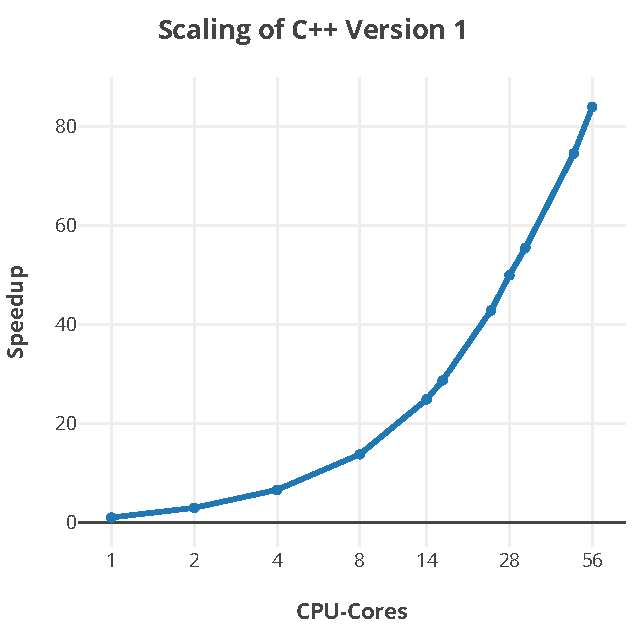
\includegraphics[width=0.32\paperwidth]{mandelbrot/assets/mandelbrot_7-scaling.pdf}
        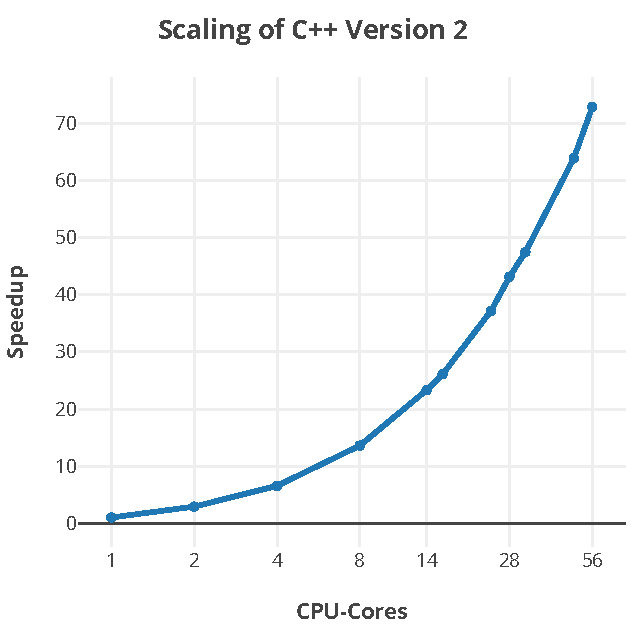
\includegraphics[width=0.32\paperwidth]{mandelbrot/assets/mandelbrot_8-scaling.pdf}
        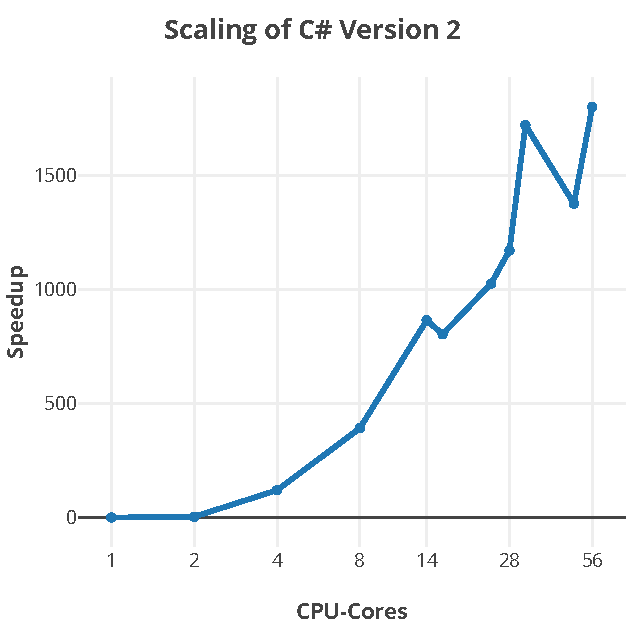
\includegraphics[width=0.32\paperwidth]{mandelbrot/assets/mandelbrot-cs-scaling.pdf}
    }
    \caption{Scaling of the C++ Version 1 (left), 2 (middle) and C\# Version 2 (right)}
    \label{fig:scaling}
\end{figure}


\section{Conclusion}
\label{sec:conclusion}

The given problem was understood and the critical parts of the \ms{} calculations are identified and, if possible, optimized. Using the provided code base, loops and optimization targets are located and analyzed to provide the foundation of two optimization strategies. The second strategy is implemented and proves to be scalable, which is elucidated in the evaluation. However, due to the increased workload of the \textit{I/O threads}, the parallel code amount can not be calculated accurately using Amdahl's law.


\end{document}